%%%%%%%%%%%%%%%%%%%%%%%%%%%%%%%%%%%%%%%%%
% Zotero proxy
% origin date: 19 Aug 2017
% revised: 
% To modify: 
%     latexila /usr/local/share/texmf/tex/latex/texMemo/texMemo.cls
%%%%%%%%%%%%%%%%%%%%%%%%%%%%%%%%%%%%%%%%%

% When you first open the template, compile it from the command line with the 
% commands below to make sure your LaTeX distribution is configured correctly:
% Re-run to get TOC
% 1) pdflatex Retaining_Volunteers_20171103
% 2) biber Retaining_Volunteers_20171103
% 3) pdflatex Retaining_Volunteers_20171103 x 2

% run LaTex -> PDF (Latexmk) in LaTexilla to get .idx file
% then
% 1) pdflatex Retaining_Volunteers_20171103
% 2) makeindex Retaining_Volunteers_20171103.idx -s StyleInd.ist
% 3) biber Retaining_Volunteers_20171103
% 4) pdflatex Retaining_Volunteers_20171103 x 2

\documentclass[letterpaper,11pt]{texMemo}

\usepackage[utf8]{inputenc}
\usepackage[T1]{fontenc}
\usepackage{graphicx}
\usepackage{hyperref}
\usepackage{amsmath}
\usepackage{amsthm}
\usepackage{amssymb}
\usepackage{comment}
\usepackage{csquotes}
\usepackage{outlines}

% BIBLIOGRAPHY
\usepackage[american]{babel} 
\usepackage[style=apa,
            sorting=nyt,
            sortcites=true,
            autopunct=true,
            hyperref=true,
            maxcitenames=2,
            mincitenames=1,
            maxbibnames=10,
            backref=true,
            doi=false,
            url=false,
            backend=biber]{biblatex}
\addbibresource{/home/bruce/Desktop/BibLatex/My_Library_20170125.bib} % BibTeX bibliography file
%\defbibheading{bibempty}{}
\DeclareLanguageMapping{american}{american-apa}    % avoid yearmonthday problems


\memoto{Karen Ciccone}
\memofrom{Bruce Marron}
\memosubject{Zotero proxies in Firefox}
\memodate{\today}
\logoa{
\includegraphics[width=0.35\textwidth]{graphics/ncstate.jpeg}}
\logob{
\includegraphics[width=0.35\textwidth]{graphics/DEAL_lab.jpg}}


\begin{document}
\maketitle
Hey Karen! Thought I'd pass on what I discovered about Zotero library proxies in Firefox (and try out a Latex memo style with our new logos!). Sure enough, Zotero (in Firefox) was keyed to my old Portland State proxy. To make the switch to NCSU's library proxy, I did the following:
\begin{outline}[enumerate]
\1 Change Zotero proxy settings in Firefox
\2 In Firefox, Open menu $\rightarrow $ Add-Ons $\rightarrow $ Zotero Preferences $\rightarrow $ Proxies
\2 In the pop-up box, 'Configured Proxies' note the current proxy, click on the current proxy, and select the Edit button
\3 Change \verb!Hostname: Multi-site!
\3 Change \verb!Scheme: http://%h.proxy.lib.ncsu.edu/%p!
  
\begin{figure} [!htbp]
  \begin{center}
    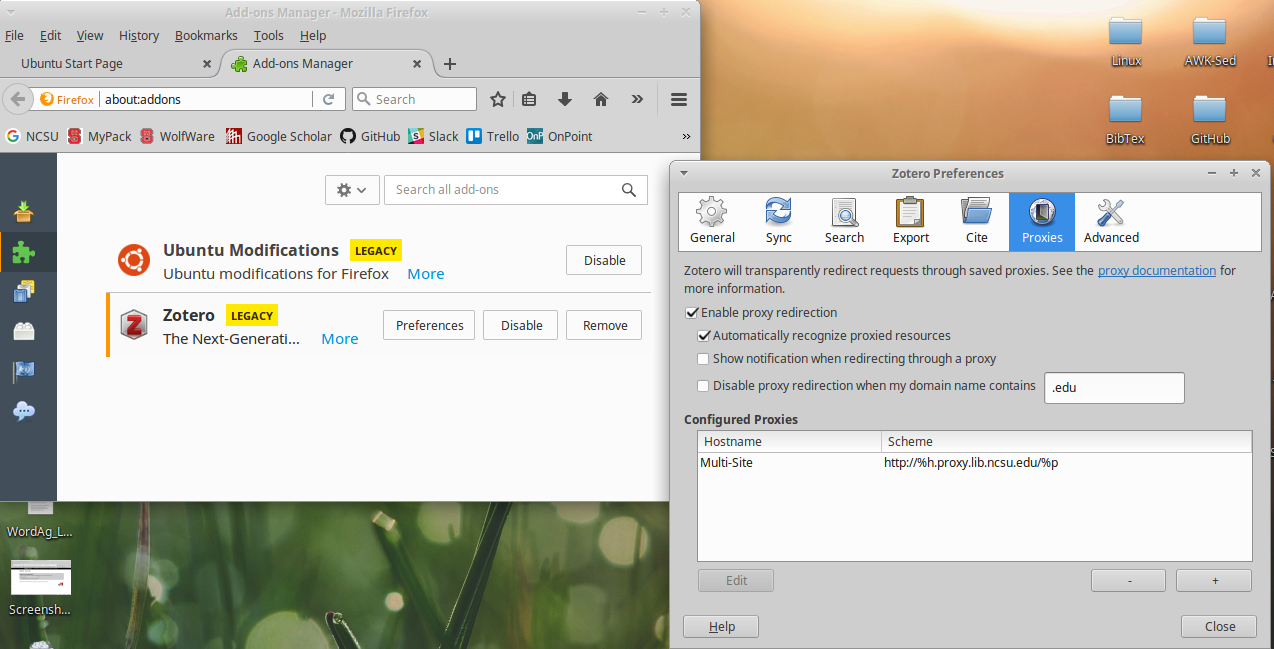
\includegraphics[width=0.75\textwidth]{graphics/Screenshot_2017-08-19_09-08-59.png}
    \caption{Zotero proxy settings.}
    \label{fig:}
  \end{center}
\end{figure}

\2 Close and exit all boxes, tabs, and windows to return to your Firefox homepage

\newpage
\1 Login to Google Scholar via NCSU library and authenticate
\2 Go to \verb!https://www.lib.ncsu.edu/articles/google-scholar/!
\2 Click to select the Google Scholar homepage
\2 A pop-up box appears, "In order to access a Resource on host 'prox.lib.ncsu.edu' you must authenticate yourself."
\2 Select "NC State Unity Users" and if desired, check "Remember selection for this web browser session"

\begin{figure} [!htbp]
  \begin{center}
    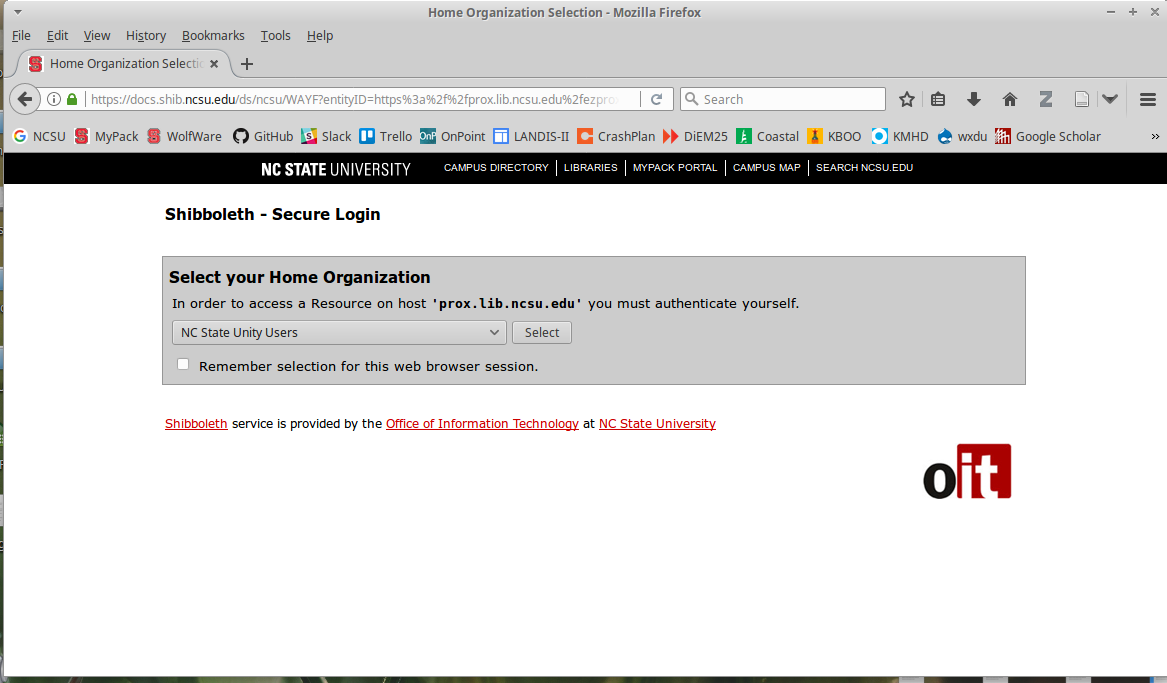
\includegraphics[width=0.75\textwidth]{graphics/Screenshot_2017-08-19_09-02-30.png}
    \caption{"Authenticate yourself"}
    \label{fig:}
  \end{center}
\end{figure}

\2 Login to Shibboleth as usual.

\newpage
\1 Set Zotero to redirect to the new proxy
\2 After login, a notice in the Firefox toolbar will state, "Zotero detected that you are accessing this website through a proxy. Would you like to automatically redirect future requests to scholar.google.com through login.prox.lib.ncsu.edu?"
\3 Click on "Enable" and then "Add proxy"

\begin{figure} [!htbp]
  \begin{center}
    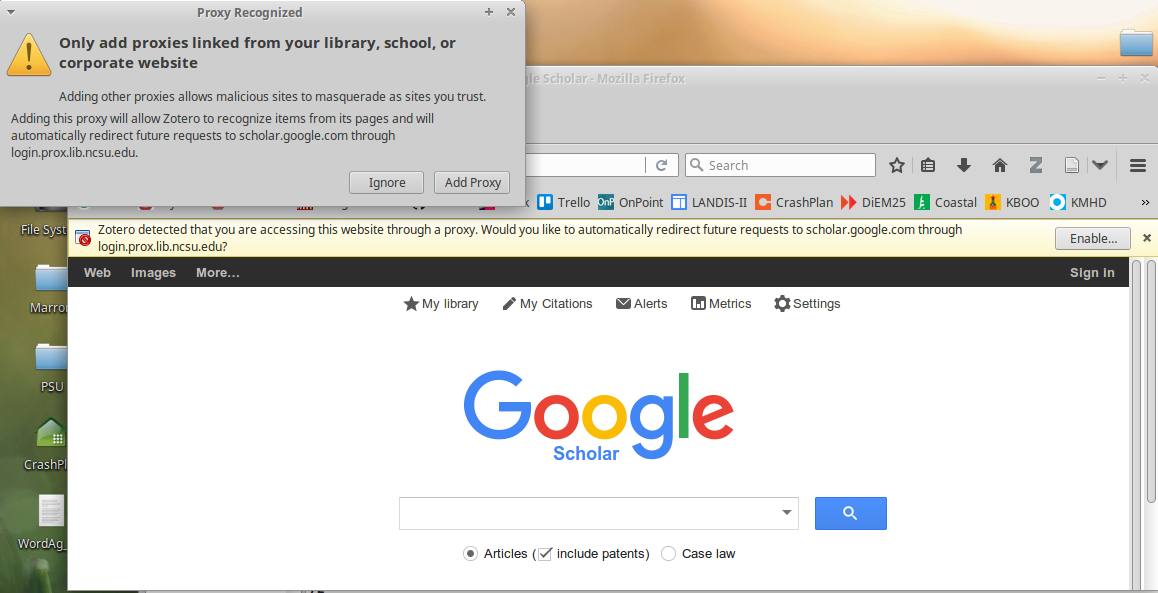
\includegraphics[width=0.75\textwidth]{graphics/Screenshot_2017-08-19_12-33-31.png}
    \caption{Enable the proxy.}
    \label{fig:}
  \end{center}
\end{figure}

\end{outline}

Voila!

\autocite{karl_give_2008}

% ----------------------------------------------------------------------------------------
% 	BIBLIOGRAPHY
% ----------------------------------------------------------------------------------------
          

\printbibliography


\end{document}
